\section{Span, Linear Independence}
\subsection{Span}
Throughout this section, let $\mathbb{K}$ be a field. We constrain ourselves to work in $V$, a $\mathbb{K}$-vector space.
\definition{Span}{
	Let $k$ be some positive integer. Let  $\{v_1, v_2, ... , v_k\}\subseteq V$. The \textbf{span} of $\{v_1, v_2, ... , v_k\}$ is denoted as \[
	\textrm{span}(v_1,v_2,...,v_k)
	\]
	and is the \textit{smallest} subspace of $V$ containing $\{v_1, v_2, ... , v_k\}$.
	If $\textrm{span}(v_1,v_2,...,v_k) = V$, we say that $\{v_1,v_2,...,v_k\}$ is a spanning set of $V$, or $\{v_1,v_2,...,v_k\}$ spans $V$.
}
The \textit{smallest} here means that if another subspace $W$ contains $\{v_1,...,v_k\}$, $W$ cannot be a subset of $\textrm{span}(v_1,...,v_k)$. How do we know such a subspace exists? We can take the intersection of all the subspaces containing $\{v_1,...,v_k\}$ \[
\textrm{span}(v_1,...,v_k) = \bigcap_{W \textrm{ subspace containing } \{v_1,...,v_k\}} W
\]
which is a subspace containing $\{v_1,...,v_k\}$ and is a subset of all other subspaces containing $\{v_1,...,v_k\}$. We know $V\subseteq V$ is a subspace containing $\{v_1,...,v_k\}$, so the intersection is between at least one set and is thus well-defined.
\proposition{
     The span of $\{v_1, v_2,\ ... , v_k\}\subseteq V$ is 
    all linear combinations of the vectors in the set:
    \[\textrm{span}\{v_1, v_2,\ ... , v_k\} = \{c_1v_1 + c_2v_2 + ... + c_kv_k | c_1, c_2, ... c_k \in \mathbb{K}\}\]
}
\begin{proof}
	We first show $\textrm{span}\{v_1, v_2, ... , v_k\} \supseteq \{c_1v_1 + c_2v_2 + ... + c_kv_k | c_1, c_2, ... c_k \in \mathbb{K}\}$. That is, for every $W$ subset containing $v_1,...,v_k$, $W$ must also contain $c_1v_1+...+c_kv_k$. \\
	We now show $\textrm{span}\{v_1, v_2, ... , v_k\} \subseteq \{c_1v_1 + c_2v_2 + ... + c_kv_k | c_1, c_2, ... c_k \in \mathbb{K}\}$. The right side is a set that nonempty, is closed under addition and scalar multiplication, and contains $v_1= 1v_1+0v_2+...+0v_k$,...,$v_k=0v_1+...+0v_{k-1}+1v_k$. Therefore, it is one of the $W$ subspaces whose intersection is used to construct the span.
\end{proof}

% insert examples including what the span of one, two, etc. vectors is

It can be difficult to how to think about what the span of a set of vectors looks like, though it is also important to develop
an intuition for it as more complex techniques are developed. It is also important to consider what vectors span a given subspace.

\example{
	Sketch, in $\reals^3$, the following spans: span$(\{\vec{i}\})$, span$(\{\vec{i},\vec{j}\})$, span$(\{\vec{i},\vec{j},\vec{k}\})$.
}
\todo write something here\\
\subsection{Linear Independence}
Thinking geometrically in the previous example, the span of one vector is one-dimensional (a line), the span of two vectors is two-dimensional (a plane),
and the span of three vectors is three-dimensional (the whole 3D space). Specifically,
we can give a correspondence between the linear combination of $k$ vectors $\{c_1{v}_1,...,c_k{v}_k\}$and a point in $\reals^k$ as \[
	c_1{v}_1+c_2{v}_2+...+c_k{v}_k \sim \begin{bmatrix}
		c_1 \\ c_2\\ ...\\ c_k
	\end{bmatrix}
\]
Assuming this correspondence works, the geomtry of the span should resemble $\reals^k$.
Unfortunately, this is not always true, for instance, consider the following counterexample:
\example{
	Sketch, in $\reals^3$, $\textrm{span}(\vec{i},\vec{k},\vec{i}+2\vec{k})$.
}
\todo

What went wrong here is that the third vector $\vec{i}+2\vec{k}$ is already a linear combination of the first two, and so this vector is `redundant' in the set.
More precisely, $(1,2,0)$ and $(0,0,1)$ give the same linear combination of the three vectors, so the correspondence fails. We thus want to answer the following question:
\begin{quotation}
	Given a set of $k$ vectors $\{{v}_1,...,{v}_k\}$, when do these vectors span the full $k$-dimensions?
	If they do not span the full $k$ dimensions, how many dimensions do they span?  
\end{quotation}

We already have one candidate criterion for spanning the full dimensions.
\definition{Linear Independence}{
	Let $\{{v}_1,...,v_k\}\subseteq V$. We say that $v_1,...,v_k$ are \textbf{linearly independent} if every linear combination of $v_1,...,v_k$ is unique. Precisely, if there are $c_1,...,c_k, d_1,...,d_k\in\mathbb{K}$ such that \[
	c_1v_1+c_2v_2+...+c_kv_k = d_1v_1+d_2v_2+...+d_kv_k,
	\]
	then \[c_1=d_1, c_2=d_2,...,c_k=d_k.\]
	If $\{v_1,...,v_k\}$ is not linearly independent, we say that it is \textbf{linearly dependent}.
}
This might be very tricky to verify, so we would like some simplier definitions for linear independence.
\proposition{
	%\iffalse
	The following are equivalent definitions for linear independence:
	\begin{itemize}
		\item (*) There is only one way to make $0_V$. i.e. If $c_1v_1+...+c_kv_k=0_V$, then $c_1=c_2=...=c_k=0$.
		\item (**) If $k\geq2$, there is no way to express one vector as a linear combination as the others. i.e. For all $1\leq j\leq k$, $v_j\notin \textrm{span}(v_1,...,v_{j-1},v_{j+1},...,v_k)$.
	\end{itemize}
	%\fi
}
\begin{proof}%[ Linear independent  $\iff$ (*)]
	We first show the original definition of linear independence implies (*).
	We already have one way to create the zero vector as a linear combination of the set, namely\[
	0v_1+0v_2+...+0v_k=0_V.
	\] By definition of linear independence, this is the only way to create the zero vector.
	\\
	We now show (*) implies the original definition of linear independence. Let (*) hold. Then if \[
	c_1v_1+...+c_kv_k=d_1v_1+...+d_kv_k,
	\] then rearranging the terms we will get \[
		(c_1-d_1)v_1+...+(c_k-d_k)v_k = 0_V.
	\]
	Since there is only one way to make $0_V$, it must be that $c_1-d_1=c_2-d_2=...=c_k-d_k=0$, or $c_1=d_1,...c_k=d_k$. This matches our original definition of linear independence.
\\
	Now we set $k\geq 2$ and show the equivelence of (*) and (**).
	We now show (*) implies (**).  
	Let (*) hold, and $v\in\textrm{span}(v_1,...,v_{j-1},v_{j+1},...,v_{k})$.
	Then $v-v_j$ is a linear combination of $v_1,...,v_k$ that is not $0v_1+...+0v_k$ as the coefficient before $v_j$ is $-1$. So that \[
		v-v_j\neq 0_V \implies v\neq v_j.
	\]
	What we have shown is that everything in $\textrm{span}(v_1,...,v_{j-1},v_{j+1},...,v_{k})$ is not $v_j$. Which means $v_j\notin \textrm{span}(v_1,...,v_{j-1},v_{j+1},...,v_k)$.
	\\
	One end of chapter exercise will guide you through the direction (**) implies (*).
\end{proof}
\todo introduce contraposition and contradiction?

We now have an informal statement: \textit{If the set is not linearly independent, then the dimension of the span must be less than k}.
This is because from (**), at least one of the vectors is redundant, so that we can remove that vector and still produce the same span with $k-1$ vectors.
\subsection{Basis}

Finally, we have a special notion when the set $\{{v}_1,\ldots,v_k\}$ span $V$ and are linearly independent. This means that every $v\in V$ is
\textit{a unique combination} of $\{{v}_1,\ldots,v_k\}$.
\definition{Basis}{
	Let $\{{v}_1,...,v_k\}\subseteq V$. We say that $v_1,...,v_k$ form a \textbf{basis} for $V$ if
	they span $V$ and are linearly independent. 
}
\example{
	In $\reals^n$, the standard basis vectors $\vec{e}_1,\vec{e}_2,\ldots,\vec{e}_n$ are a basis. This is why
	we call them the standard basis. 
}
\definition{Dimension}{
	If a vector space $V$ has a finite basis, we call $V$ finite dimensional. Else we call $V$ infinite dimensional. 
}
\begin{remark}
	It is true that every basis of a vector space has the same number of elements, so we can assign a number (or infinity) to the dimension of a vector space. However, we will have to prove that later when we develop more technology.
\end{remark}
\theorem{Every Vector Space has a Basis}{
	Let $V$ be a $\mathbb{K}$ vector space. Then $V$ has a basis.
}
\textcolor{red}{Understanding this proof is optional.} Our main hurdle here is that vector spaces are not necessarily `small' to work with.
For instance, $\reals^n$ is finite dimensional, so is in some sense small. But now consider the following real vector space:\[
	\tilde{V}=\{(a_1,a_2,a_3,\ldots) \ | \ a_j\in\reals \}
\]
Each element in this set is an infinite sequence of real numbers, and addition/scaling is entry-wise.
You may argue that the infinite set $S=\{(1,0,0,\ldots), (0,1,0,\ldots),(0,0,1,\ldots),\ldots\}$ could be a basis. However,
they do not span $\tilde{V}$. To show that, I claim that the subset \[
U = \{(a_1,a_2,a_3,\ldots)\in\tilde{V} \ | \textrm{ only finitely many $a_j$'s are non zero}\}
\]
is a subspace of $\tilde{V}$. It is a strict subset of $\tilde{V}$, contains the zero vector $(0,0,0,\ldots)$ and is closed
under addition and $\reals$-scaling.
It also contains $S$ as each element in $S$ has $1$ (thus finitely many) non-zero element(s).
Thus $\textrm{span}(S)\subseteq U \subset \tilde{V}$.

To circumvent this, this proof requires the use of the axiom of choice, which we will give a statement below.
\definition{Axiom of Choice}{
	The \textbf{Axiom of Choice} is one of the axioms in Zermelo-Frenkel (ZFC) Set theory. Its statement is as follows:
	\begin{quotation}
		Let $I$ be a set, $(S_i)_{i\in I}$ be an indexed family of non-empty sets. Then there exists an indexed set $(s_i)_{i\in I}$ such that
		$s_i\in S_i$ for each $i\in I$.
	\end{quotation}
	Colloquially, it means there is a ``choice function'' that allows you to pick an element from each of the non-empty $S_i$'s.
}
\begin{remark}
	What we lose from the Axiom of Choice is that the choice function is non-constructive. This means that we know that something exists without knowing
	exactly how to construct it. The Axiom of Choice also leads to weird consequences, for example the Banach-Tarski paradox states that you can
	rearrange the points of a solid 3D ball to make two solid 3D balls, each having the same size as the original. (!)
	While some mathematicians do not accept the Axiom of Choice and adopt ZF (ZFC without \textit{C}hoice), it generally makes our lives easier.
\end{remark}
From the Axiom of Choice, one can derive Zorn's Lemma. This is the optional part.
\theorem{Zorn's Lemma}{
	Assume the Axiom of Choice. Let $S$ be a partially ordered set, that is, there is a comparison function $\leq$ for some pairs of elements.
	Then if for every ascending chain in $S$ \[
	s_1,s_2,\ldots \in S \textrm{ such that } s_1\leq s_2 \leq s_3 \leq \ldots,
	\]There is some $t\in S$ such that $s_j\leq t$, then $S$ has a maximal element (nothing is bigger than $S$).
}
\begin{remark}
	The example of Zorn's Lemma is as follows:
	Let $S$ contain subsets of $V$. We have a partial ordering on $S$ using inclusion.\[
	A\leq B \textrm{ if } A\subseteq B.
	\] 
	If for every chain $A_1\subseteq A_2 \subseteq A_3\subseteq\ldots$ we can find $B\in S$ that contains all the $A_j$'s, then $S$ has a maximal element.
\end{remark}
\begin{proof}[Proof of Every Vector Space has a Basis]
	Let $S = \{L\subseteq V \ | \textrm {L is linearly independent}\}$. We give $S$ the partial ordering with respect to set inclusion. We first show $S$ has a maximal element using Zorn's Lemma.

	For each ascending chain $L_1\subseteq L_2\subseteq \ldots$, we claim $U=\bigcup_i L_i$ is a linearly independent set.
	We verify it directly: Let $v_1,\ldots, v_k\in U, c_1,\ldots,c_k\in\mathbb{K}$,
	and $\sum_{i} c_i v_i = 0_{V}$.
	We know that for each $1\leq i\leq k$ there $L_{a_i}$ such that $v_i\in L_{a_i}$. Take $a=\max_i a_i$.
	Then $v_i\in L_a$. Because $L_a$ is a linearly independent set, it must be that $c_1=\ldots=c_k=0$.
	
	Now we apply Zorn's Lemma to get that there is a maximal element $M\in S$. We claim $\textrm{Span}(M)$.
	If not, we can find $v\in V$ such that $v\notin\textrm{Span}(M)$, but then this means $M\cup\{v\}$ is a linearly independent set.
	This contradicts that $M$ is a maximal element.
\end{proof}
\exercises
\begin{exerciselist}
	\item \textit{(**) $\implies$ (*) in linear independence} Let $c_1v_1+\ldots + c_kv_k=0_V$. If $c_1\neq 0$, argue that $v_1\in \textrm{span}(v_2,...,v_k)$, thus this case cannot happen and $c_1=0$. Then show that $c_j=0$ for all $j$, and thus the $v_j$'s are linearly independent.
	\item Write down a basis for the vector space of all polynomials of degree $k$ or less. 
\end{exerciselist}
\section{Systems of Linear Equations}
As we alluded to earlier, many types of vector spaces are in some way very similar to $\reals^n$. For instance, the span of a set of $k$ linearly independent real-vectors has a natural correspondence to $\reals^k$.
With the blind faith that everything here can generalize nicely back to abstract vector spaces, we limit ourselves again back to talking about $\reals^n$.\\
Here, we introduce a new notation to write linear combiantions, as $c_1v_1+...+c_kv_k$ is very cumbersome.
\definition{Matrix}{
	Let $m$ and $n$ be positive integers. An $m\times n$ \textbf{matrix} is a rectangular array of $m$ rows and $n$ columns in the form \[
		\begin{bmatrix}
			c_{1,1} & c_{1,2} & \ldots & c_{1,n} \\
			c_{2,1} & c_{2,2} & \ldots & c_{2,n} \\
			\vdots & & \ddots  \\
			c_{m,1} & c_{m,2} &\ldots & c_{m,n} 
		\end{bmatrix}\]
	where each $c_{i,j}$ is an \textbf{entry} of the matrix.
	We denote the set of all $m\times n$ matrices with real entries $M_{m\times n}(\reals)$. In general, we have $M_{m\times n} (\mathbb{K})$ for entries in the field $\mathbb{K}$.
}
\begin{notation}
	Suggestively, we can write an $m\times n$ matrix as \[
	\begin{bmatrix}
		\vec{v}_1 & \vec{v}_2 & ... & \vec{v}_n
	\end{bmatrix}
	\]
	where each $\vec{v}_j\in\reals^m$ is written as a column vector\[
	\begin{bmatrix}
		c_{j,1} \\ c_{j,2}\\ \vdots \\ c_{j,m}
	\end{bmatrix}.
	\]
	If we want to think of the matrix by its entries, we can also write the matrix as \[
	\{c_{i,j}\}
	\]
\end{notation}
\definition{Matrix-vector Product}{
	Let \[
	A =\begin{bmatrix}
			\vec{v}_1 & \vec{v}_2 & ... & \vec{v}_n
		\end{bmatrix}
	\] be an $m\times n$ matrix, and \[
	\vec{b}=\begin{bmatrix}
		b_1 \\ b_2 \\ \vdots\\b_n
	\end{bmatrix} \in \reals^n.
	\]
	The product of $A$ and $\vec{b}$ is evaluated as \[
		A\vec{b} = b_1\vec{v}_1+ b_2\vec{v}_2 + ...+ b_n\vec{v}_n.
	\]
}\example{
	Let $M=\begin{bmatrix}
		\vec{e}_1 & \vec{e}_2 &\ldots &\vec{e}_n
	\end{bmatrix}$ be an $n\times n$ matrix.
	Compute $M\vec{x}$ for any $\vec{x}\in\reals^n$.
}
The computation is not too difficult. We can follow the definition to get \[
	M\vec{x}=x_1\vec{e}_1 + x_2\vec{e}_2 + \ldots + x_n\vec{e}_n = \vec{x}.
\]
Basically, multiplying a vector with the matrix with columns $\vec{e}_1,\ldots,\vec{e}_n$ does not change the vector. This should not be surprising, since the corresponding system of equations for $M\vec{x}=\vec{b}$ is \begin{align*}
	x_1 &= b_1\\ x_2 &=b_2 \\ \vdots\\x_n&=b_n
\end{align*}
\definition{Identity Matrix}{
	We denote the $n\times n$ \textbf{identity matrix} by \begin{align*}
		I_n \defeq \begin{bmatrix}
			\vec{e}_1 & \vec{e}_2 & \ldots&\vec{e}_n
		\end{bmatrix}=\begin{bmatrix}
			1 & 0 & 0& \ldots & 0\\
			0 & 1 & 0 & \ldots & 0\\
			0 & 0 & 1 & \ldots & 0\\
			\vdots & && \ddots&\\
			0 & 0 & 0& \ldots & 1
		\end{bmatrix}.
	\end{align*}
		
	
}
\proposition{
	The matrix-vector product satisfies the following properties. Let $c\in\reals,\vec{x}_1,\vec{x}_2\in\reals^n, A\in M_{m\times n}(\reals)$, then \begin{itemize}
		\item $A(\vec{x}_1+\vec{x}_2)=A\vec{x}_1+A\vec{x}_2$,
		\item $A(c\vec{x}_1)= c(A\vec{x}_1)$.
	\end{itemize}
}
This means that the matrix-vector product preserves linear combinations.
$A(c_1\vec{x}_1+...+c_k\vec{v}_k)=c_1A\vec{x}_1+...+c_kA\vec{x_k}$.

\example{
	Determine if the vectors \[
	\vec{v}_1=\begin{bmatrix}
		1\\0\\1
	\end{bmatrix}
	,\vec{v}_2=\begin{bmatrix}
		1\\1\\0
	\end{bmatrix},
	\vec{v}_3=\begin{bmatrix}
	0\\1\\1
	\end{bmatrix}
	\] are linearly independent.
}
Recalling the definition for linear independence, we solve for 
\[
\begin{bmatrix}
	1&1&0\\
	0& 1 & 1\\
	1& 0 & 1
\end{bmatrix} \begin{bmatrix}
	c_1 \\ c_2\\c_3
\end{bmatrix} = \begin{bmatrix}
	0\\0\\0
\end{bmatrix}.
\]
This is a compact way to express the system
\begin{align*}
	c_1 + c_2 + 0 &= 0 \\
	 0+  c_2 +  c_3 &= 0\\
	c_1+ 0+c_3 &= 0
\end{align*}
There is a very slick way to find the solution (which involves adding all three equations together), but let us solve this methodically. This method is known as elimination, which involves isolating variables, and thus reducing the complexity of the system one by one.
\\
First, we look at the first equation and isolate $c_1=-c_2$. Now we can look replace all instances of $c_1$ in the second and third equation with $-c_2$, giving us \begin{align*}
	c_1 + c_2 + 0 &= 0 \\
	0 +  c_2 +  c_3 &= 0\\
	0 - c_2 +c_3 &= 0
\end{align*}
If we look at just the second and third equations, these only have two variables, so we have effectively decreased the complexity of the system by 1. Whatever we get from the second and third equations, we can substitute back into the first to get $c_1$.
Now, we repeat for the second equation, $c_2=-c_3$, and replacing all instances of $c_2$ we have \begin{align*}
	c_1 + 0 - c_3 &= 0 \\
	0 +  c_2 +  c_3 &= 0\\
	0 + 0 + 2c_3 &= 0
\end{align*}
The third equation now is just an equation in one variable, so we can go ahead and solve \begin{align*}
	c_1 + 0 - c_3 &= 0 \\
	0 +  c_2 +  c_3 &= 0\\
	0 + 0 + c_3 &= 0
\end{align*}
and replace all instances of $c_3$ with $0$ to get 
\begin{align*}
	c_1 + 0 + 0 &= 0 \\
	0 +  c_2+  0 &= 0\\
	0 + 0 + c_3 &= 0
\end{align*}
or $c_1=c_2=c_3=0$. This is indeed a solution to the system, so we can now conclude that these vectors are indeed linearly independent.
If we condense the systems back to matrices (concatenating the $3\times 3$ matrix and the vector on the right)  we get 
\begin{align*}
	\left[
	\begin{array}{ccc|c}
		1&1&0&0\\
		0&1&1&0\\
		1&0&1&0
	\end{array} \right] \rightarrow
	\left[\begin{array}{ccc|c}
		1&1&0&0\\
		0&1&1&0\\
		0&-1&1&0
	\end{array}\right] \rightarrow
	\left[\begin{array}{ccc|c}
		1&0&-1&0\\
		0&1&1&0\\
		0&0&2&0
	\end{array}\right]
	\rightarrow
	\left[\begin{array}{ccc|c}
		1&0&0&0\\
		0&1&0&0\\
		0&0&1&0
	\end{array}\right]
\end{align*}
\example{
	Determine the solutions to the system of equations \begin{align*}
		0 + 2x_2-x_3 &= 1\\
		x_1 - x_2 + x_3 &= 0 \\
		x_1 + x_2 + 2x_3 & = 1
	\end{align*}
}
The first equation here does not let us isolate $x_1$, but we can simply exchange the first two equations to get \[
\begin{bmatrix}[ccc|c]
	1 & -1 & 1 & 0\\
	0&2&-1&1\\
	1& 1 & 2 & 1\\
\end{bmatrix}
\]
We want to remove any dependence of $x_1$ for the other two equations, so we can subtract the first equation from the third to get \[
	\begin{bmatrix}[ccc|c]
		1 & -1 & 1 & 0\\
		0&2&-1&1\\
		0& 2 & 1 & 1\\
	\end{bmatrix}
\]
We divide the second equation by $2$, add this equation to the first, and subtract from the third.
\[
	\begin{bmatrix}[ccc|c]
		1 & -1 & 1 & 0\\
		0&1&\frac{-1}{2}&\frac{1}{2}\\
		0& 2 & 1 & 1\\
	\end{bmatrix} \sim
	\begin{bmatrix}[ccc|c]
		1 & 0 & \frac{1}{2} & \frac{1}{2}\\
		0&1&\frac{-1}{2}&\frac{1}{2}\\
		0& 2 & 1 & 1\\
	\end{bmatrix}
	\sim
	\begin{bmatrix}[ccc|c]
		1 & 0 & \frac{1}{2} & \frac{1}{2}\\
		0&1&\frac{-1}{2}&\frac{1}{2}\\
		0& 0 & 2 & 0\\
	\end{bmatrix}
\]
Finally, we divide the third equation by $2$, and remove all other entries of the third column.
\[
	\begin{bmatrix}[ccc|c]
		1 & 0 & 0& \frac{1}{2}\\
		0&1&0&\frac{1}{2}\\
		0& 0 & 1 & 0\\
	\end{bmatrix}
\]
So the solution is $x_1=1/2, x_2=1/2, x_3=0$.
\subsection{Elementary Row Operations and Row Echelon Form}
By how we manipulated the equations in the previous examples, we motivate these operations on matrices.

\definition{Elementary Row Operations and row equivalence}{
	The following operations on a matrix $A\in M_{m\times n}$ are known as \textbf{elementary row operations}:\begin{enumerate}
		\item \textit{(Row Swap)} Exchange any two rows.
		\item \textit{(Scaling)} Multiply a row by a \textbf{non-zero} constant.
		\item \textit{(Sum)} Add a multiple of a row to another row.
	\end{enumerate}
	Let $B\in M_{m\times n}$. We say that $A$ is \textbf{row equivalent} to $B$ if $A$ can be transformed into $B$ By
	applying a sequence elementary row operations. We denote this equivalence by $A\sim B$.
}
\begin{remark}
	We can group the big set of $M_{m\times n}(\reals^n)$ into classes, where each class contains matrices that are row equivalent to each other.
\end{remark}
\proposition{
	Elementary row operations are invertible. That is, if $A\sim A'$ after applying an elementary row operation,
	$A'\sim A$ through applying a (possibly different) row operation.
}
\proposition{
	An $m\times n$ matrix can be viewed as a system of $m$ equations in $n-1$ variables using the representation in the previous two examples.
	In this representation, row equivalent matrices have the same solution sets.
}
The proof is not very enlightening. It boils down to checking that each of the three elementary row operations do not change the solution set of the corresponding linear system, so a sequence of them will not change the solution sets.
The key takeaway from this is that we can reduce the complexity of the matrix through elementary row operations. Let us define the `simple'
forms of a matrix you can get through row operations.

\definition{Row Echelon Form and Pivots}{
	A matrix is in \textbf{row echelon form} if \begin{itemize}
		\item Rows with all zero entries are on the bottom.
		\item For each row having non-zero entries, the first non-zero entry is on the right of the first non-zero entry of the row above.
	\end{itemize}
	In row echelon form, the first non-zero entry of a row is called a \textbf{pivot}.
	Colloquially, the non-zero entries form a ``staircase'' like shape.
}
\example{
	The following matrix is in row echelon form:\[
	\begin{bmatrix}
		1 & * & * & * & * \\
		0 & 0 & 2 & * & * \\
		0 & 0 & 0 & 1 & * \\
		0 & 0 & 0 & 0 & 0
	\end{bmatrix}
	\]
	The pivots of this matrix, from the first row, are $1$, $2$ and $1$.
}
In most cases, reducing a matrix into the row echelon form is ``good enough'' to find solutions. Start from the bottom row, and substitute variables go up.
However, one problem with working with row echelon form is that a matrix is row equivalent to many matrices in row echelon form, so we want some `super' row echelon form
that is unique to each matrix.
\definition{Reduced Row Echelon Form}{
	A matrix is in \textbf{Reduced Row Echelon Form}(rref) if \begin{itemize}
		\item It is in row echelon form.
		\item All pivots are equal to $1$.
		\item Every pivot is the only non-zero entry in its column.
	\end{itemize}
}
\example{
	The following matrix is in reduced row echelon form:\[
	\begin{bmatrix}
		1 & * & 0 & 0 & * \\
		0 & 0 & 1 & 0 & * \\
		0 & 0 & 0 & 1 & * \\
		0 & 0 & 0 & 0 & 0
	\end{bmatrix}
	\]
}
By how we defined the reduced row echelon form, we cannot find two distinct matrices in reduced row echelon form that are also row equivalent. This guarantees
that a matrix is row equivalent to at most one reduced row echelon form matrix.
\theorem{Existence and Uniqueness of Reduced Row Echelon Form}{
	Let $A \in M_{m\times n}(\reals)$. Then there exists a unique $A'\in M_{m\times n}(\reals)$ such that $A'$ is in reduced
	row echelon form and $A \sim A'$. We define $A'$ to be the \textbf{reduced row echelon form} of $A$, and denote
	\[
		A' = \textrm{rref}(A).
	\]
}

\begin{proof}
	Formalizing our steps in the previous examples, we have an algorithm for reducing a matrix into rref.

	\begin{algorithm}
		\caption{Gaussian-Jordan Reduction of $A\in M_{m\times n}(\reals^n)$}
		
			$i\gets 1$, $j\gets 1$
			\While {$j\leq n$}{
				\For {$k$ in $i\ldots m$} {
					\Comment*[l]{Find a row with non-zero entry in that column}
					\If {$a_{k,j}\neq 0$}{
						 swap(row $i$, row $k$) \Comment*[r]{Move row $k$ to the top row}
						 row $i \gets 1/a_{i,j} \times $ row $i$ \Comment*[r]{Normalize pivot to $1$}
						\For {$l$ in $1\ldots m$, $l\neq i$}{
							 row $l \gets$ row $l$ - $(a_{l,j}\times$ row $i)$ \Comment*[r]{all other entries in the same column $=0$}
						}
						$i\gets i+1$ \Comment*[r]{Next row with pivot goes to the row below}
						Break
					}
				}
				 $j\gets j+1$ \Comment*[r]{check pivot in next column}
			}
	\end{algorithm}
	\todo Gaussian-Jordan Reduction
\end{proof}
\example{
	Compute \[
	\textrm{rref}\left(\begin{bmatrix}
		something here lol
	\end{bmatrix}\right)
	\]
}
\subsection{Recovering solutions from rref}
%\subsubsection*{No solutions}
%There are no solutions when the system of equations is inconsistent. In rref, this corresponds to creating a row that says $0=1$.

\subsubsection*{Producing one solution}
Let us consider a general matrix in rref:\[
	\begin{bmatrix}[c c c c c|c]
		1& *& * &* &*& a\\
		0& 0 & 1 &* &*& b\\
		0& 0 & 0 &0 &1& c\\
		0& 0& 0 & 0 &0& d\\
	\end{bmatrix}
\]
If $d\neq0$, the rref form will imply $d$ is a pivot and thus equal to $1$.
So the last equation requires $0=1$, which means it has no solutions!

Now we set $d=0$, so $a,b,c$ can be anything.
Regardless of the * entries, we can set for the columns with pivots, $x_1=a, x_3=b, x_5=c$, 
and for the columns corresponding to non-pivots, $x_2=x_4=0$. We thus have
\theorem{Solutions to linear systems}{
	Let $A\in M_{m\times n}(\reals), \vec{b}\in\reals^m$, the system of equations described by
	$A\vec{x}=\vec{b}$ has\[
	\begin{cases}
		\textrm{No solutions, if rref}\left(\left[A | \vec{b}\right]\right)\textrm{ has a pivot in the last column,}\\
		\textrm{At least one solution, if the last column does not have a pivot}
	\end{cases}
	\]
	Moreover, if the latter case holds, one solution (a particular solution) can be constructed
	from the rref by just solving the columns of rref$\left(\left[A | \vec{b}\right]\right)$
	with pivots, and setting the variables corresponding to non-pivot columns to $0$.
}


\subsubsection*{Producing all solutions}
Now, suppose $A\vec{x}=\vec{b}$ has at least one solution. It can have infinitely many solutions! We want to describe this set of solutions without actually
writing infinitely many vectors. One starting point is to see what properties this set satisfies. One starting point 
would be to guess that the set $\{\vec{x}\in\reals^n | A\vec{x}=\vec{b}\}$ is a subspace of $\reals^n$.
This is generally not true, as every subspace contains $\vec{0}_{\reals^n}$, and since $A\vec{0}_{\reals^n}=\vec{0}_{\reals^m}$,
the only possible way this could be a subspace is when $\vec{b}=\vec{0}_{\reals^m}$.\\

We thus start with the solution set to $A\vec{x}=\vec{0}$.
\definition{Nullspace}{
	Let $A\in M_{m\times n}(\reals)$. The \textbf{nullspace} of the A, denoted $N(A)$, is the set of all solutions $\vec{x}$ 
	for $A\vec{x}=\vec{0}$. i.e. \[
		N(A)=\{\vec{x}\in\reals^n | A\vec{x}=\vec{0}_{\reals^m}\}.
	\]
}
\proposition{
	Let $A\in M_{m\times n}(\reals)$. \[
	N(A)= N (\textrm{rref}(A)).\]
}
\begin{proof}
	\todo
\end{proof}
This allows us to limit the discussion of nullspaces to when $A$ is in rref.

It turns out that the nullspace is a subspace. This is why we tend to like systems of linear equations where the right hand side is all zero.
We call these systems \textbf{homogeneous}, and the solutions to homogeneous linear systems form a subspace.
\theorem{Nullspace is a Subspace}{
	Let $A\in M_{m\times n}(\reals)$. $N(A)$ is a subspace of $\reals^n$.
}
\begin{proof}
	\todo zero is in here, closed under addition and multiplication
\end{proof}
\example{
	Find the solutions to the system represented by 

	\[
		\begin{bmatrix}[c c c c c | c]
			1& 0& 1& 0 & -3 & 0\\
			0& 1& 1& 0 & 4 & 0\\
			0& 0& 0& 1 & -2 & 0
		\end{bmatrix}.
	\]
	Express the answer in the form of the span of a set of linearly independent vectors.
}
Let us start with the last variable $x_5$ and work our way towards $x_1$.
There is no equation that fixes $x_5$, so let $x_5 = s$ for some $s\in\reals$.
Then the last equations fixes $x_4 = 2s$. 

Again, we do not have an equation that fixes $x_3$, so let $x_3=t$ for some $t\in\reals$.
This will force (from the second equation) $x_2= -t-4s$ and (from the first equation) $x_1 = -t+3s$.

Our solution vector $(x_1,x_2,x_3,x_4,x_5)$ thus has the form \[
\begin{bmatrix}
	-t+3s\\ -t-4s\\ t\\ 2s\\ s
\end{bmatrix}= s\begin{bmatrix}
	3 \\ -4 \\ 0 \\ 2 \\ 1
\end{bmatrix} + t \begin{bmatrix}
	-1 \\ -1 \\ 1 \\0 \\0
\end{bmatrix}
\]
This describes exactly the span of the vectors \[
	\begin{bmatrix}
		3 \\ -4 \\ 0 \\ 2 \\ 1
	\end{bmatrix} ,
	\begin{bmatrix}
		-1 \\ -1 \\ 1 \\0 \\0
	\end{bmatrix}.
\]
To confirm these vectors are linearly independent, notice the third entry of the first vector and the fifth entry of the second vector is $0$.

From this example, we have an algorithm to solve for the nullspace as a span of vectors.
\begin{algorithm}
\caption{Generating the Nullspace of Matrix $A$}

	$A\gets \textrm{rref}(A)$\\
	 $S\gets$ empty set\\
	\For{each column $j$ without a pivot} {
		 $\vec{v} \gets \vec{e}_j$\\
		\For{each row $i$ with a pivot}{
			 Locate pivot of row $i$ in column $k$\\
			 $\vec{v} \gets \vec{v} - a_{i,j} \vec{e}_k$\\
		}
		Add $\vec{v}$ to S\\
	 }
	\Return span$(S)$
\end{algorithm}
\\
This is what we did in the previous example, except written in pseudocode.
The idea is that each column without a pivot denotes a free variable, while each column with a pivot is a fixed by the free variables.
This is what we do in lines $5$ to $8$, after fixing our free variable to be $1$, we subtract from the fixed variables. 
In particular,\textit{ there is at most one solution if every column has a pivot}.
Now we return back to solving $A\vec{x}=\vec{b}$. We showed that the solutions do not form a subspace. However, these solutions are related to the nullspace.

\example{
	Find the solutions to the system represented by 

	\[
		\begin{bmatrix}[c c c c c | c]
			1& 0& 1& 0 & -3 & 1\\
			0& 1& 1& 0 & 4 & 2\\
			0& 0& 0& 1 & -2 & 3
		\end{bmatrix}.
	\]
}
Similar to computing nullspace, let us start with the last variable $x_5$ and work our way towards $x_1$.
There is no equation that fixes $x_5$, so let $x_5 = s$ for some $s\in\reals$.
\textcolor{red}{Then the last equations fixes $x_4 = 3+2s$}. 

Again, we do not have an equation that fixes $x_3$, so let $x_3=t$ for some $t\in\reals$.
This will force (from the second equation) \textcolor{red}{$x_2= 2-t-4s$} and (from the first equation) \textcolor{red}{$x_1 = 1-t+3s$}.

Our solution vector $(x_1,x_2,x_3,x_4,x_5)$ thus has the form \[
\begin{bmatrix}
	1-t+3s\\ 2-t-4s\\ t\\ 3+2s\\ s
\end{bmatrix}= \begin{bmatrix}
	1\\2\\0\\3\\0
\end{bmatrix}+s\begin{bmatrix}
	3 \\ -4 \\ 0 \\ 2 \\ 1
\end{bmatrix} + t \begin{bmatrix}
	-1 \\ -1 \\ 1 \\0 \\0
\end{bmatrix}
\]
This is the nullspace, but shifted by the vector $(1,2,0,3,0)$.
\proposition{
	Let $\vec{x}_1,\vec{x}_2\in\reals^n$ be solutions to $A\vec{x}=\vec{b}$.Then\[
		(\vec{x}_1-\vec{x}_2)\in N(A).
	\] 
}
\begin{proof}
	We compute directly that $A(\vec{x}_1-\vec{x}_2)=\vec{b}-\vec{b}=\vec{0}$.
\end{proof}
\corollary{
	Let $\vec{v}$ be \textit{one} solution to $A\vec{x}=\vec{b}$. Then all the solutions of $A\vec{x}=\vec{b}$ is exactly\[
	\{\vec{v}+\vec{n}|\vec{n}\in N(A)
		\}.\]
}
This means we only need one solution (particular solution), and the nullspace (homogeneous) solution to solve any matrix.
This one solution can be obtained by setting all the `free variables' in the solution to zero, and solving for all the pivots.

When producing solutions, the number of pivots of rref$(A)$ is important. Let us define the number of pivots to be the rank of $A$. 
\definition{Rank}{
	Let $A\in M_{m\times n }(\reals)$. We define the \textbf{rank} of $A$\[
		\textrm{rank}(A) = \textrm{the number of pivots in rref}(A).
	\]
}
We can thus formulate having zero, one or infinitely many solutions in terms of the number of pivots.
\proposition{
	Let $A\in M_{m\times n}(\reals), \vec{b}\in\reals^m$, the system of equations described by
	$A\vec{x}=\vec{b}$ has\[
	\begin{cases}
		\textrm{At least one solution, if rank}\left(\left[A | \vec{b}\right]\right) = \textrm{rank}(A)\\
		\textrm{At most one solution, if rank} (A)=n.
	\end{cases}
	\]
}
Going back to why we started solving linear systems, we want to find a test to see if the vectors are linearly independent, or if some vector is in the span of a set of vectors.
Writing $A=[\vec{v}_1 \ \ldots \ \vec{v}_n]$, $A\vec{x}=\vec{b}$ having at least one solution means $\vec{b}\in\textrm{span}(\vec{v}_1,\ldots,\vec{v}_n)$,
and if $A\vec{x}=\vec{0}$ has exactly one solution, the $\vec{v}_j$'s are linearly independent.
\theorem{Rank and span/linear independence correspondence}{
	Let $A=[\vec{v}_1 \ \ldots \ \vec{v}_n]\in M_{m\times n}(\reals)$, $\vec{b}\in\reals^m$.
	Then \begin{itemize}
		\item  rank$\left(\left[A | \vec{b}\right]\right) = \textrm{rank}(A) \iff$ $\vec{b}\in\textrm{span}(\vec{v}_1,\ldots,\vec{v}_n)$. 
		\item rank$(A)=m\iff\textrm{span}(\vec{v}_1,\ldots,\vec{v}_n)=\reals^m$.
		\item rank$(A)=n\iff\{\vec{v}_1,\ldots,\vec{v}_n\}$ is linearly independent. 
	\end{itemize}
}
\begin{remark}
	This is the first time we used the $\iff$ symbol. This means `if and only if', or `iff' for short.
	`$A\iff B$' means that if A holds, then B holds. And if B holds, A holds. 
	For instance, `more than 99\% guarantees an A' means \begin{quotation}
		You have more than 99\% in this course $\implies$ you get an A
	\end{quotation}
	But you can still get an A without reaching this score, for instance a 95\% could get an A too.
	An if and only if statement (for a strict grading class) would look more like \begin{quotation}
		The threshold for A in this class is a 90\%.
	\end{quotation}
	so \{You get A\} $\iff$ \{You get 90+\%\}.
\end{remark}
\begin{proof}
	The first and third statements are evident from the definitions of span and linear independence.

	To show the second statement, we first prove the $\implies$ direction.
	Let $\vec{b}\in\reals^m$, then reducing $[A|\vec{b}]$ would give $m$ pivots in the first $n$ columns, so there cannot be a pivot in the final column.
		(or else, we would have $m+1$ pivots in a matrix with only $m$ rows). Therefore, the system has a solution.

	For the $\impliedby$ direction, we can reverse all the elementary operations from $A$ to $\textrm{rref}(A)$ to get from
	$[\textrm{rref}(A)|\vec{e}_m]$ to $[A|\vec{w}]$ for some $\vec{w}\in\reals^m$. This system of equations has no solution.
\end{proof}

Something amazing also happens when the vectors are a basis (recall it means both linearly independent and spans $\reals^m$).

The second and third statements forces $m=\textrm{rank}(A)=n$, so $A$ is a square matrix. The vectors span $\reals^m$ iff they are linearly independent.
\theorem{This One/ That One}{
	Let $A\in M_{n\times n}(\reals)$, and write $A=[\vec{v}_1\ldots\vec{v}_n]$.
	Then the following are equivalent.
	\begin{thatonethmlist}
		\item $\{\vec{v}_n,\ldots,\vec{v}_n\}$ form a basis.
		\item $\{\vec{v}_n,\ldots,\vec{v}_n\}$ are linearly independent.
		\item $\{\vec{v}_n,\ldots,\vec{v}_n\}$ span $\reals^n$.
		\item The system of equations $A\vec{x}=\vec{b}$ has exactly one solution for each $\vec{b}\in\reals^n$.
		\item The system of equations $A\vec{x}=\vec{b}$ has at least one solution for each $\vec{b}\in\reals^n$.
		\item The system of equations $A\vec{x}=\vec{b}$ has at most one solution for each $\vec{b}\in\reals^n$.
		\item Rank$(A)=n$.
		\item rref$(A)$ has a pivot in every column.
		\item rref$(A)$ has a pivot in every row.
		\item $N(A)=\{\vec{0}\}$.
	\end{thatonethmlist}
}\begin{remark}
	This One Theorem goes by many names: Invertibility Theorem, Inverse Matrix Theorem, Inverse Function Theorem, and (my favorite) Amazingly Awesome Theorem by Prof. Ca\~nez.
	Despite the lack of standardization, it is covered in every linera algebra course in some form or another.
	I'm putting it as `That One Theorem', so when you quote `this follows from That One Theorem' everyone will understand which one you are talking about. 
\end{remark}
\begin{remark}
	This One Theorem is still incomplete. We will build towards more equivalences.
\end{remark}
\exercises
\begin{exerciselist}
	\item Determine if the following sets of vectors are linearly dependent or independent. If they are not linearly independent, generate the set of homogenous solutions to the corresponding linear system. \begin{enumerate}[label=(\alph*)]
		\item $\{(1,2,3), (0,1,1),(1,1,2)\}$
		\item $\{\vec{e}_1,\vec{e}_2,\vec{e}_5\}\subset\reals^7$
		\item 
	\end{enumerate}
	\item Let $m>n$. Show that every set of $m$ vectors in $\reals^n$ is not linearly independent. Show that every set of $n$ vectors in $\reals^m$ does not span $m$. Thus show that every basis for $\reals^n$ has $n$ vectors.
	\item Let $\{v_1,...,v_k\}\subset V$. Show that exactly one of the following statements hold: \begin{enumerate}[label=(\alph*)]
		\item For every $v\in \textrm{span}(\{v_1,...,v_k\})$, there is exactly one way to write $v$ as a linear combination of $v_1,...,v_k$.
		\item For every $v\in \textrm{span}(\{v_1,...,v_k\})$, there is more than one way to write $v$ as a linear combination of $v_1,...,v_k$.
	\end{enumerate}
	\item \textit{Every vector space has a basis (weaker version)} This is a weaker statement of \href{thm:2.14}{Every Vector Space has a Basis}. To get around this, we use a finiteness assumption that our vector space $V$ is a subspace of $\reals^n$.\begin{enumerate}[label=(\alph*)]
		\item Suppose that our subspace is $\{\vec{0}\}$. Show that this is spanned by the empty set. The empty set is (vacuously) linearly independent*, so we have a basis. \textit{* all elements of an empty set satisfy any condition}
		\item Now suppose $S=\{\vec{v}_1,\ldots,\vec{v}_k\}\subset V\subseteq \reals^n$. Show that this is a linearly independent set in $V$ if and only if this is a linearly independent set $\reals^n$, so we can call it linearly independent without worrying about which vector space we work in.
		\item Let $S$ be linearly independent. If $\textrm{span}(S)=V$ this will be a basis for $V$. Else show that there is some $\vec{v}_{k+1}\in V$ such that the set $S+\{\vec{v}_{k+1}\}$, so you can extend $S$ to a bigger linearly independent set.
		\item Show that the previous process terminates, i.e. you cannot add in infinitely vectors and still make $S$ linearly independent. Therefore, it stops at some $k$ where $\textrm{span}(\{\vec{v}_1,\ldots,\vec{v}_k\})=V$.
	\end{enumerate}
	\item Show that every subset of a linearly independent set is linearly independent.
	\item 
\end{exerciselist}

\section{Linear Transformations}
Matrix-vector multiplication preserve linear combinations. Let us name this property.
\definition{Linear Transformation}{
	Let $V$ and $W$ be $\mathbb{K}$-vector spaces. A function $f: V\to W$ is a \textbf{linear transformation} if it preserves
	linear combinations. Namely, for every $c\in\mathbb{K}, \vec{v}_1,\vec{v}_2\in V$,\begin{itemize}
		\item $f(\vec{v}_1+\vec{v}_2)=f(\vec{v}_1)+f(\vec{v}_2)$,
		\item $f(c\vec{v}_1)=cf(\vec{v}_1)$.
	\end{itemize}
}
Many functions in the wild are linear transformations. This includes the functions we have introduced so far.
\example{
	The following are examples linear transformations:
	\begin{enumerate}
		\item A matrix $A\in M_{m\times n}(\reals)$ admits a linear transformation $F:\reals^n\to \reals^m$ by \[
			F(\vec{x})=A\vec{x}.
		\]
		\item Let $\vec{v}\in\reals^n$. $f(\vec{x})=\vec{v}\cdot\vec{x}$ is a linear transformation from $\reals^n\to\reals$. The projection Proj$_{\vec{v}}$ is a linear transformation from $\reals^n\to\reals^n$.
		\item Let $\vec{v}\in\reals^3$. $f(\vec{x})=\vec{v}\times\vec{x}$ is a linear transformation from $\reals^3\to \reals^3$.
		\item Recall that the set of polynomials $f(x)$ is a real vector space. The differentiation operator $\frac{d}{dx}$ is a linear transformation from the set of polyomials to itself.
		\item Integration over a bounded interval $\int_{a}^{b}$ is a linear transformation from the space of integrable functions to $\reals$.
	\end{enumerate}
}

\proposition{
	Let $U,V,W$ be $\mathbb{K}$-vector spaces, and $T_1:U\to V, T_2:U\to V, T_3:V\to W$ be linear transformations, then the following are also linear transformations: \begin{itemize}
		\item $f_1:U\to V$, $f_1(\vec{x}) = T_1(\vec{x})+T_2(\vec{x})$
		\item $f_2:U\to V$, $f_2(\vec{x})=c T_1(\vec{x})$ for any $c\in\mathbb{K}$
		\item $f_3:U\to W$, $f_3(\vec{x})= T_3(T_1(\vec{x}))$.
	\end{itemize}
}
The first example of linear transformation given $A\vec{x}$ is a very general type of linear transformation.
The punchline is that it is \textbf{the} example of a linear transformation.
\theorem{Matrix Representation of Linear Transformation}{
	Let $T:\reals^n \to \reals^m$ be a linear transformation. Then there is a matrix $A\in M_{m\times n}$ such that for all $\vec{x}\in\reals^n$,
	\[
		T(\vec{x})=A\vec{x}.
	\]
	We denote this matrix the \textbf{matrix representation} of $T$.
}
\begin{remark}
	Importantly, this theorem is only applicable for $\reals^n\to\reals^m$, both are \textbf{finite dimensional}.
	Some linear functions work with infinite dimensional (we will give a definition later) vector spaces. Intuitively, this means the analogous
	`standard basis vectors' is an infinite set $\{\vec{e}_1,\vec{e}_2,\ldots\}$. 
\end{remark}
Before we head to the details of the proof, here is the idea behind our constuction.
Let us suppose that this matrix exists; how do we compute each entry of the matrix?
The trick is to think of the matrix as $\begin{bmatrix}
	\vec{w}_1 & \vec{w}_2 & ... & \vec{w}_n
\end{bmatrix}$.
We can get a linear combination of these to equal any of the $\vec{w}_j$'s. Namely, using the standard basis vectors,
$A\vec{e}_j=\vec{w}_j$. Since $A\vec{e}_j=T(\vec{e}_j)$That means our matrix must be in the form \[
	\begin{bmatrix}
		T(\vec{e}_1) \ T(\vec{e}_2) \ \ldots \ T(\vec{e}_n)
	\end{bmatrix} .
\]
Now all we need to do check that this matrix works.
\begin{proof}
	We claim that the matrix $A=\begin{bmatrix}
		T(\vec{e}_1) \ T(\vec{e}_2) \ \ldots \ T(\vec{e}_n)
	\end{bmatrix}$ satisfies $T(\vec{x})=A\vec{x}$.
	Let $\vec{x}\in \reals^n$. Then $\vec{x}=\sum_{i=1}^{n} x_i\vec{e}_i$.
	So that by linearity, \[
	T(\vec{x}) = \sum_{i=1}^{n} x_i T(\vec{e}_i) = A \begin{bmatrix}
		x_1 \\ x_2 \\ \vdots \\ x_n
	\end{bmatrix} = A\vec{x}.
	\]
\end{proof}	
\subsection*{More intuition behind the proof}
We can also think of a linear transformation geometrically.
Let us track the transformation $T:\reals^2\to\reals^2$ that sends $T(\vec{e}_1)= (2,1)$ and $T(\vec{e}_2)=(-1,1)$.
\begin{figure}[h]
	\centering
	\begin{subfigure}[l]{0.15\textwidth}
		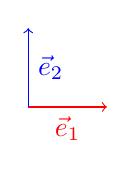
\begin{tikzpicture}
			
			\draw [->,color=red] (0,0)--(1,0) node[midway, below]{$\vec{e}_1$} ;
			\draw [->,color=blue] (0,0)--(0,1) node [right,midway]{$\vec{e}_2$};
			\end{tikzpicture}
	\end{subfigure}
	\centering
	\begin{subfigure}{0.3\textwidth}
		\begin{tikzpicture}
	
			\draw [->,thick] (0,0)--(4,0) node[midway, above]{$T$};
			\node (A) at (5,0){};
			\end{tikzpicture}
	\end{subfigure}
	\begin{subfigure}[r]{0.4\textwidth}
		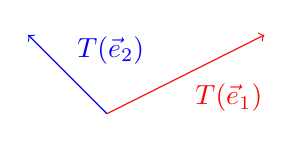
\begin{tikzpicture}
	
			\draw [->,color=red] (0,0)--(2,1) node[midway, below right ]{$T(\vec{e}_1)$} ;
			\draw [->,color=blue] (0,0)--(-1,1) node [above right ,midway]{$T(\vec{e}_2)$};
			\end{tikzpicture}
	\end{subfigure}
\end{figure}
Let us only consider the integer lattice points for now. If we start at $(a,b)$, meaning from the origin, we take $a$ steps right and $b$ steps up. In our transformed plane, we need to take $a$ steps in $(2,1)$ and $b$ steps $(-1,1)$ by linearity. We can geometrically track the place of these lattic points using a grid.
\begin{figure}[h]
	\begin{subfigure}[l]{0.4\textwidth}
		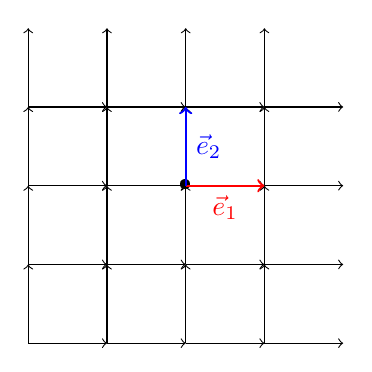
\begin{tikzpicture}
			\draw (0,0) node{\textbullet};
			\foreach \i in {-2,...,1}{
				\foreach \j in {-2,...,1}{
					\draw [->,thin] (\i,\j)--(\i+1,\j);
					
					\draw [->,thin] (\i,\j)--(\i,\j+1);
				}
			}
			\draw [->,color=red,thick] (0,0)--(1,0) node[midway, below]{$\vec{e}_1$} ;
			\draw [->,color=blue,thick] (0,0)--(0,1) node [right,midway]{$\vec{e}_2$};
			\end{tikzpicture}
			\caption{Original grid}
	\end{subfigure}
	\begin{subfigure}[r]{0.6\textwidth}
		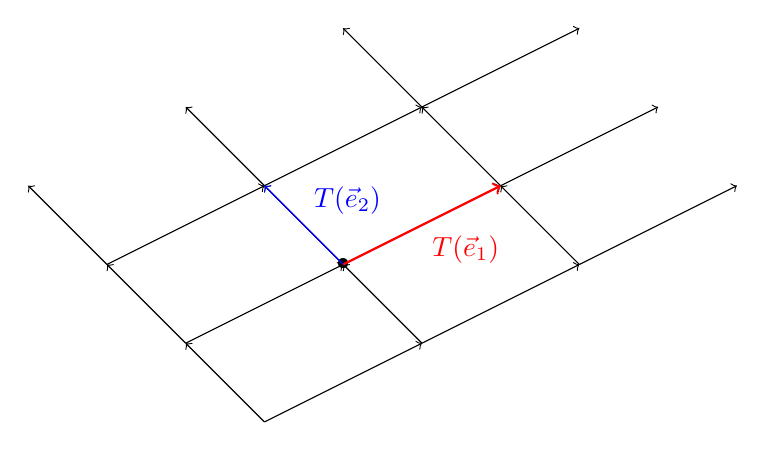
\begin{tikzpicture}
			\draw (0,0) node{\textbullet};
			\foreach \i in {-1,...,1}{
				\foreach \j in {-1,...,1}{
					\draw [->,thin] (\i*2-\j,\j+\i)--(\i*2-\j+2,\i+\j+1);
					
					\draw [->,thin] (\i*2-\j,\j+\i)--(\i*2-\j-1,\i+\j+1);
				}
			}
			\draw [->,color=red,thick] (0,0)--(2,1) node[midway, below right ]{$T(\vec{e}_1)$} ;
			\draw [->,color=blue] (0,0)--(-1,1) node [above right ,midway,thick]{$T(\vec{e}_2)$};
			\end{tikzpicture}
			\caption{Transformed grid}
	\end{subfigure}
\end{figure}
This is just a change of our coordinate system. As long as we know where the standard basis vectors go (or any basis goes), it is enough to know the whole linear transformation. The construction is you 1. decompose any vector into the linear combination of the basis vectors, then 2. add up the corresponding linear combination of the transformed basis vectors. \textbf{This intuition of linear transformations being a shift in coordinates is very useful}, and helps transform abstract problems in linear algebra back to concrete geometry. 
\example{
	Express the linear transformations of the dot product, cross product, and projection as matrix-vector multiplications.
}
\textbf{Dot Product: }Let $\vec{v}=(v_1,\ldots,v_n)\in\reals^n$. Then $\vec{v}\cdot\vec{e}_j=v_j$. So \[\vec{v}\cdot\vec{x} = \begin{bmatrix}
	v_1 & v_2 &  \ldots & v_n
\end{bmatrix}\vec{x}\].

\textbf{Cross Product} Let $\vec{v}=(v_1,v_2,v_3)\in\reals^n$. Then \[
	\vec{v}\times\vec{x} = \begin{bmatrix}
		0 & -v_3 & v_2\\
		v_3 & 0 & -v_1\\
		-v_2 & v_1 & 0
	\end{bmatrix}\vec{x}
\]

\textbf{Projection} Let $\vec{v}=(v_1,\ldots,v_n)\in\reals^n$. Then \[
	\textrm{Proj}_{\vec{v}}(\vec{x})=\frac{1}{|\vec{v}|^2}\begin{bmatrix}
		v_1 v_1 & v_1 v_2 & \ldots & v_1 v_n \\
		v_2 v_1 & v_2 v_2 & \ldots & v_2 v_n \\
		\vdots & & \ddots & \\
		v_n v_1 & v_n v-2 & \ldots & v_n v_n
	\end{bmatrix}\vec{x}
\]
where multiplication of matrix by scalar is entry wise.
\example{
	Let $T:\reals^m\to\reals^n$, $S:\reals^n\to\reals^p$. Let $A\in M_{m\times n}, B\in M_{n\times p}$ be the matrix representations of $S$ and $T$ respectively.
	We know that the function $F:\reals^m \to \reals^p$ defined by $F(\vec{x})=S(T(\vec{x}))$ has a matrix representation. Compute this matrix.
}
The computation is not very interesting. However, you will do this until the day you drop ISP.
If we write $A=\begin{bmatrix}
	\vec{x}_1 & \ldots & \vec{x}_m
\end{bmatrix}, \vec{b}_j\in\reals^n$, then for each $\vec{e}_j\in\reals^m$ we have $A\vec{e}_j=\vec{x}_j$.
So that \[
S(T(\vec{e}_j))= S(A\vec{e}_j) = S(\vec{x}_j) = B(\vec{x}_j).
\]
The matrix is \[
\begin{bmatrix}
	B\vec{x}_1 & B\vec{x}_2 & \ldots & B\vec{x}_m
\end{bmatrix}.
\]
Now, if we forcefully write the linear transformations in matrices, we get $S(T(\vec{x}))= BA\vec{x}$. This allows us
to define the product of matrices.
\definition{Matrix Operations}{
	Let $\alpha \in\reals$, $A=\{a_{i,j}\},B=\{b_i,j\}\in M_{m\times n}(\reals)$, $C=\{c_{i,j}\}\in M_{n\times p}(\reals)$.
	We define the addition of matrices \[
	A+B=\{a_{i,j}+b_{i,j}\},
	\]
	the pointwise addition of each entry. We define the scaling of a matrix \[
	\alpha A = \{\alpha a_{i,j}\},
	\]
	the pointise scaling of each entry. We also define the product of matrices\[
	AC = \left\{\sum_{k=1}^{n}a_{i,k}c_{k_j}\right\}.
	\]
}
\begin{remark}
	The definition of matrix product is equivalent to what we got from getting the matrix from the composition of functions.
	The only difference is that we are composing a function the other way from $\reals^p\to\reals^n\to\reals^m$.
\end{remark}
\begin{remark}
	There is a mnenomic to memorize the formula for matrix product $AB$. It involves putting $A$ on the bottom left and $B$ on the top right, like so:

	\[
	\begin{array}{cc}
		&\begin{bmatrix}
			b_{1,1} & \ldots & b_{1,p}\\
			\vdots & \ddots&\\
			b_{n,1} & \ldots & b_{n,p}
		\end{bmatrix}\\
		\begin{bmatrix}
			a_{1,1} & \ldots & a_{1,n}\\
			\vdots & \ddots&\\
			a_{m,1} & \ldots & a_{m,n}
		\end{bmatrix}	& \begin{bmatrix}\\
			\textrm{product goes here}\\
			\\
		\end{bmatrix}
	\end{array}
	\]
	The product of an $m\times n$ and an $n\times p$ matrix is an $m\times p$ matrix. To find the $i,j$'th entry of the product,
	locate the $i$-th row on matrix $A$ (left) and the $j$-th column on matrix $B$ (top). Treating the row and column as vectors with $n$ entries, the dot product is the $i,j$-th entry of the product.
\end{remark}
\begin{remark}
	Viewing a column vector as a $n\times 1$ matrix, you can verify that the matrix-vector product is compatible with the products of two matrices.
\end{remark}

\proposition{
	The matrix operations satisfy the following properties:\\
	\textbf{Addition: } Let $A,B,C\in M_{m\times n}(\reals)$, then: \begin{itemize}
		\item \textit{(Associativity)} $A+(B+C)=(A+B)+C$.
		\item \textit{(Commutativity)} $A+B=B+A$.
		\item \textit{(Identity)} The zero matrix $0_{m\times n}$ satisfies $A+0_{m\times n}=A$.
	\end{itemize}
	\textbf{Scaling: } Let $\alpha,\beta\in\reals, A,B \in M_{m\times n}(\reals)$, then:\begin{itemize}
		\item \textit{(Associativity)} $\alpha(\beta)A = (\alpha\beta)A$.
		\item \textit{(Distributivity)} $(\alpha+\beta)(A+B) = \alpha A + \alpha B + \beta A + \beta B$.
	\end{itemize}
	\textbf{Multiplication: } Let $A,B \in M_{m\times n}(\reals),C,D\in M_{n\times p}(\reals), E \in M_{p\times q}(\reals)$.\\
	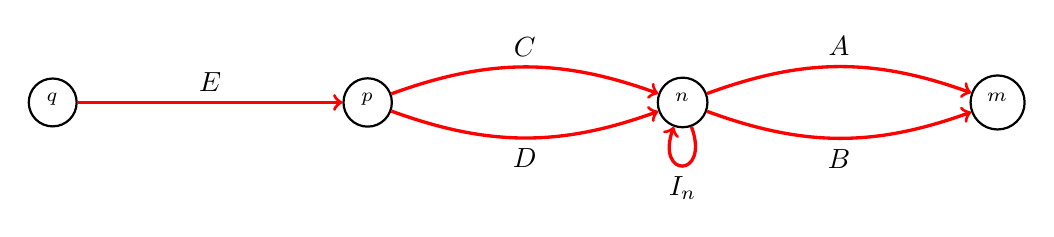
\begin{tikzpicture}
		\begin{scope}[every node/.style={circle,thick,draw}]
			\node (A) at (0,0) {$\reals^q$};
			\node (B) at (4,0) {$\reals^p$};
			\node (C) at (8,0) {$\reals^n$};
			\node (D) at (12,0) {$\reals^m$};
		\end{scope}
	
\begin{scope}[
	every edge/.style={draw=red,very thick}]
\path [->] (A) edge node [above,midway]{$E$} (B);
\path [->] (B) edge [bend left=20] node [above,midway]{$C$} (C);
\path [->] (B) edge [bend right=20]node [below,midway]{$D$} (C);

\path [->] (C) edge [in=-110, out=-70,looseness=8]node [below,midway]{$I_n$} (C);
\path [->] (C) edge [bend left=20] node [above,midway]{$A$} (D);
\path [->] (C) edge [bend right=20] node[below,midway] {$B$} (D);
\end{scope}
	\end{tikzpicture}\\
	Then \begin{itemize}
		\item \textit{(Associativity)} $A(CE)=(AC)E$.
		\item \textit{Compatibility with Scaling} $A(\alpha C)=\alpha(AC) = (\alpha A)(C)$.
		\item \textit{(Distributivity)} $(A+B)(C+D) = AC+AD+BC+BD$.
		\item \textit{(Identity)} The identity matrix $I_n = \begin{bmatrix}
			\vec{e}_1 & \vec{e}_2 & \ldots & \vec{e}_n
		\end{bmatrix}$ satisfies $I_nC = C$ and $BI_n=B$.
	\end{itemize}
}
\begin{remark}
	The matrix product is generally not commutative. In fact, the product $DB$ does not make sense, because the dimensions of the matrices are not compatible!
\end{remark}
\exercises
\begin{exerciselist}
	\item Find the corresponding matrices for the following transformations: \begin{enumerate}[label=(\alph*)]
		\item 
	\end{enumerate}
	\item Find an example where \begin{enumerate}[label=(\alph*)]
		\item Two matrices $A,B\in M_{n\times n}(\reals)$ are not commutative. i.e. $AB\neq BA$.
		\item A matrix $0_{n\times n}\neq A\in M_{n\times n }(\reals)$ such that $A^k=0_{n\times n}$ for some $k>1$.
	\end{enumerate}
	\item Let $\theta,\phi\in[0,2\pi)$. Sketch how the matrix \[\begin{bmatrix}
		\cos \theta & -\sin \theta\\
		\sin \theta & \cos \theta
	\end{bmatrix}
	\] transforms the grid. Show that \[
		\begin{bmatrix}
			\cos \theta & -\sin \theta\\
			\sin \theta & \cos \theta
		\end{bmatrix}
		\begin{bmatrix}
			\cos \phi & -\sin \phi\\
			\sin \phi & \cos \phi
		\end{bmatrix}
		=
		\begin{bmatrix}
			\cos (\theta+\phi) & -\sin (\theta+\phi)\\
			\sin (\theta+\phi) & \cos (\theta+\phi)
		\end{bmatrix}
	\]
	and thus the set of matrix in this form are commutative. Is there a geometric argument for why these matrices must be commutative? 
	\item Run the following code in python multiple times and pinky promise that you got the correct answer.\\ \begin{lstlisting}[language=Python]
import numpy as np
matrix1=np.random.randint(-10,11,size=(3,3))
matrix2=np.random.randint(-10,11,size=(3,3))
print("Multiply these two matrices:")
print(matrix1,"\n",matrix2)
print("Confirm that the answer is the following:")
print(matrix1.dot(matrix2))\end{lstlisting}
\end{exerciselist}
\section{Surjective and Injective Linear Transformation}
\definition{Types of functions}{
	Let $f:U\to W$ be a function. We say $f$ is:
	\begin{itemize}
		\item \textbf{Surjective}, if the image of $U$ under $f$, $f(U)=W$. 
		This means for every $w\in W$, there is some $u\in U$ such that $f(u)=w$.
		\item \textbf{Injective}, if each $u \in U$ maps to a unique element in $W$.
		This means for every $u_1,u_2\in U$. If $f(u_1)=f(u_2)$, $u_1=u_2$. 
		\item \textbf{Bijective}, if $f$ is surjective and injective.
	\end{itemize}
}
\example{
	The following functions are surjective:\begin{itemize}
		\item The `extract' function $\Pi_j:\reals^n\to\reals$, defined by $\Pi_j(x_1,x_2,...,x_n)=x_j$ and extracts the $j$-th coordinate.
		\item The differentiation operator $\frac{d}{dx}$ from the space of \textbf{differentiable} functions to the space of \textbf{continuous} functions. This is because all continuous functions have antiderivatives.
		Moreover, as all derivatives are continuous, the differentiation operator is well defined.
		\item Integration over the interval $[0,1]$ sends the integrable function $g$ to the real number $\int_{0}^{1}g(x) \ dx$. This is surjective because the integral 
			of $g(x)=a$ over $[0,1]$ is $a$ for all $a\in \reals$.
	\end{itemize}
	The following functions are injective:\begin{itemize}
		\item The `pad zeros' function $\iota:\reals^n \to \reals^{n+1}$ defined by $\iota(x_1,...,x_n) = (x_1,...,x_n,0)$ and adds a $0$ to the final coordinate.
		\item The linear function $f:\reals \to \reals$ defined by $f(x)=2x$.
	\end{itemize}
	The following functions are surjective:\begin{itemize}
		\item The identity map $Id:\reals^n\to\reals^n$ defined by $Id(\vec{x}) = I_n \vec{x} = \vec{x}$.
	\end{itemize}
}
We can phrase these characterizations in of the number of solutions in $u$ that solve $f(u)=w$.
\proposition{
	\begin{itemize}
		\item $f$ is surjective $\iff$ $f(u)=w$ has \textit{at least one solution} in $u$ for each $w\in W$.
		\item $f$ is injective $\iff$ $f(u)=w$ has \textit{at most one solution} in $u$ for each $w\in W$.
		\item $f$ is bijective $\iff$ $f(u)=w$ has \textit{exactly one solution} in $u$ for each $w\in W$.
	\end{itemize}
}
When $f$ is a linear transformation from $\reals^n \to \reals^m$, it has a matrix representation $A\in M_{m\times n}(\reals)$.
To determine if $f$ is surjective, injective, or bijective, we look at the number of solutions in $\vec{x}$ for the equation $A\vec{x}=\vec{b}$
for each $\vec{b}\in\reals^m$.
\theorem{Surjectivity and solutions to linear systems}{
	Let $T:\reals^n\to\reals^m$, $A\in M_{m\times n}(\reals)$, and $T(\vec{x})=A\vec{x}$ for all $\vec{x}\in\reals^n$.
	Then the following are equivalent:\begin{enumerate}
		\item $T$ is surjective.
		\item $A(\vec{x})=\vec{b}$ is at least one solution in $\vec{x}$ for each $\vec{b}\in \reals^m$
		\item rref$(A)$ has a pivot in every row.
		\item The columns of $A$ span $\reals^m$.
	\end{enumerate}
}
\theorem{Injectivity and solutions to linear systems}{
	Let $T:\reals^n\to\reals^m$, $A\in M_{m\times n}(\reals)$, and $T(\vec{x})=A\vec{x}$ for all $\vec{x}\in\reals^n$.
	Then the following are equivalent:\begin{enumerate}
		\item $T$ is injective.
		\item $A(\vec{x})=\vec{b}$ is at most one solution in $\vec{x}$ for each $\vec{b}\in \reals^m$.
		\item rref$(A)$ has a pivot in every column.
		\item The columns of $A$ are linearly independent.
	\end{enumerate}
}
Again, something interesting happens when $T:\reals^n\to\reals^m$ is bijective.
This forces the matrix to be square, giving even more equivalences for That One Theorem.
\theorem{This One/ That One (Linear transformation cont.)}{
	Let $A=[\vec{v}_1\ldots \vec{v}_n]\in M_{n\times n}(\reals)$, and $T:\reals^n\to\reals^n$ be the unique linear transformation satisfying $T(\vec{x})=A\vec{x}$ for all $\vec{x}\in\reals^n$.
	Then the following are equivalent.
	\begin{enumerate}
		\item $\{\vec{v}_1,\ldots,\vec{v}_n\}$ form a basis.
		\\ $\vdots$
	\end{enumerate}
	
	\begin{thatonethmlist}
		\item $T$ is bijective.
		\item $T$ is surjective.
		\item $T$ is injective.
	\end{thatonethmlist}
}
\exercises